\chapter{\label{lesson10}Движение по прямой}
{\bfseries Анонс:}\\\\
Среда программирования RobotC. Подача напряжений на моторы, задержки, синхронизация моторов. Принципы оформления кода. Счетчик числа оборотов. Проблема движения по инерции.\\\\
{\bfseries Цели:}
\begin{itemize}
	\item{}{\bfseries Обучающие:} Знакомство с редактором RobotC. Освоение простейших команд и циклов. Комментирование кода.
	\item{}{\bfseries Коммуникативная:} Обучение детей работать во взаимодействии с другими учащимися (работа в группах)   и учителем.\\
\end{itemize}	
{\bfseries Ход занятия:}\\\\
\begin{tabular}{lll}
	\hyperlink{lesson10x1}{1. Организационный момент} & Презентация & (15 мин)\\
	\hyperlink{lesson10x2}{2. Практикум «Движение прямо»} & Практика & (40 мин) \\
	\hyperlink{lesson10x3}{3. «Самый точный робот»} & игра & (30 мин) \\
	\hyperlink{lesson10x4}{4. Проблемы инерционности} & Обсуждения & 15 мин)\\
	\hyperlink{lesson10x5}{5. Комментарии} & Презентация & 5 мин)\\
\end{tabular}\\\\

{\hypertarget{lesson10x1}{\blackBlueText{I. Организационный момент}}}\\\\ 

Перед началом работы каждая команда должна собрать стандартную трех колесную тележку, которую будет в дальнейшем программировать.
\clearpage
{\hypertarget{lesson10x2}{\blackBlueText{II.  Практикум «Движение прямо»}}}\\\\

Давайте напишем программу, которая заставит нашего робота ехать вперед:\\\\

{\programm
	{\slshape\bC{task main}}\rC{()}\\
	\rC{\{}\\
	\indent \bbC{motor}\rC{[\rrC{motorB}] =  \rrC{100};}\\
	\indent \bbC{motor}\rC{[\rrC{motorC}] =  \rrC{100};}\\
	\indent \bbC{wait1Msec}\rC{(\rrC{1000});}\\
	\rC{\}}\\
}\\\\

Скомпилируем ее, загрузим на робота, запустим. Видим, что робот проехал прямо 1 секунду и остановился. Что же мы приказали роботу сделать? Команда motor[motorB]=100; подает на мотор, подключенный к выходу В максимальную мощность (100 условных единиц). Мы можем написать после знака равно и 10 и 80 и даже -23, в общем, любое значение от -100 до 100.  Следующая команда подает такую же мощность на второй мотор, подключенный к выходу С. Мы включили оба двигателя, что будет если программу на этом закончить? Предложим роботу следующий код:\\\\

{\programm
	{\slshape\bC{task main}}\rC{()}\\
	\rC{\{}\\
	\indent \bbC{motor}\rC{[\rrC{motorB}] =  \rrC{100};}\\
	\indent \bbC{motor}\rC{[\rrC{motorC}] =  \rrC{100};}\\
	\rC{\}}\\
}\\\\

Ничего не происходит, такое  ощущение что программа пустая. В чем же дело? Поставим себя на место робота: он начинает исполнять программу, включает мотор В, включает мотор С и заканчивает программу. Учтем, что на каждое действие он тратит миллисекунды. Он включил моторы и тут же закончил программу, т.е. все выключил. Колеса не успевают даже дернуться. Подожди, не заканчивай так быстро! Собственно это и говорит команда wait1Msec(1000). Такая команда говорит роботу подождать столько миллисекунд, сколько указано в скобках, в нашем случае 100мс = 1с. И робот включает моторы и ждет в таком состоянии 1 секунду, т.е. едет 1 секунду, что мы и наблюдали.

{\slshape Здесь рекомендуется выделить время и дать учащимся попрактиковаться в самостоятельном написании программы. В качестве задачи учащимся может быть предложено запрограммировать трехколесную тележку так, что бы она проехала 5 метров и остановилась.}

Отлично, мы можем ехать прямо вперед любое фиксированное время. Ну или почти прямо?  Правое и левое колесо управляются разными моторами и вращаются чуть-чуть по-разному, вследствие чего робот начинает ехать не вполне ровно. Что бы управление моторами было синхронным существует следующая команда:\\\\

{\programm
	\indent \bbC{nSyncedMotors }\rC{=  \rrC{synchNone};} \indent \gC{// моторы не синхронизированы}\\
	\indent \bbC{nSyncedMotors }\rC{=  \rrC{synchВС};~~} \indent \gC{// мотор ‘C’ управляет мотором ‘B’}\\
}\\\\

А как сделать так, что б робот ехал вперед всегда, бесконечно долго? Для этого воспользуемся циклом while. While переводится с английского,  как «до тех пор пока». Формат записи такой:\\\\

\indent While(условие)\\
\indent \{\\
\indent\indent Что делать, пока это условие истинно ;\\	
\indent \}\\\\

Т.е. искомая программа «бесконечного» движения будет выглядеть так:\\\\

{\programm
	{\slshape\bC{task main}}\rC{()}\\
	\rC{\{}\\
	\indent{\slshape\bC{while}}\rC{({\slshape\bC{true}})}\\
	\indent\rC{\{}\\
	\indent\indent\bbC{motor}\rC{[\rrC{motorB}] =  \rrC{100};}\\
	\indent\indent\bbC{motor}\rC{[\rrC{motorC}] =  \rrC{100};}\\
	\indent\rC{\}}\\
	\rC{\}}\\
}\\\\

Пока условие в скобках while истинно (а оно в данном случае истинно всегда) выполняются команды в теле цикла – подавать напряжения на моторы.

Тут хочется сказать еще вот о чем. В языке RobotC пробелы, переносы строк, символы табуляции не имеют большого значения для компилятора. Там где стоит пробел, может быть перенос строки и наоборот. На самом деле 10 пробелов подряд, 2 переноса строки и ещё 5 пробелов~--- это всё эквивалент одного пробела. Пустое пространство~--- это инструмент программиста, с помощью которого можно или сделать программу понятной и наглядной, или изуродовать до неузнаваемости. Так, наша программа бесконечного движения может быть записана и следующим образом:\\\\

{\programm
	{\slshape\bC{task main}}\rC{()\{}{\slshape\bC{while}}\rC{({\slshape\bC{true})}\{}\bbC{motor}\rC{[\rrC{motorB}]=\rrC{100};}\bbC{motor}\rC{[\rrC{motorC}]=\rrC{100};}\rC{\}\}}
}\\\\	

Запись определенно стала компактнее, но гораздо менее читаемой и понятной. Поэтому, при написании программы принято следовать негласному правилу оформления:

Всегда, при начале нового блока между \{ и \} увеличивайте отступ на одинаковое число пробелов (2 или 4).

Применение этого правила превращает нашу программу в такую:\\\\

{\programm
	{\slshape\bC{task main}}\rC{()}\\
	\rC{\{}\\
	\indent{\slshape\bC{while}}\rC{({\slshape\bC{true}})}\\
	\indent\rC{\{}\\
	\indent\indent\bbC{motor}\rC{[\rrC{motorB}] =  \rrC{100};}\\
	\indent\indent\bbC{motor}\rC{[\rrC{motorC}] =  \rrC{100};}\\
	\indent\rC{\}}\\
	\rC{\}}\\
}\\\\

Тут так же разумно отметить, что в отличие от пробелов, переносов строк и табуляции символ ; которым мы заканчиваем почти каждую строчку, как раз имеет смысл для компилятора. По нему компилятор понимает, где заканчивается команда. Обратим внимание так же на то, что ; заканчивают команды, но не объявления циклов и условий (после while точку с запятой мы не ставили).

Давайте еще раз запустим программу, написанную для Практикума 6 и замерим, сколько проехал робот. Программа не поменялась, а расстояние уменьшилось, почему так?  «Сели батарейки». Когда мы говорим роботу motor[motorB]=100 , он подает на мотор максимальную мощность. Но сама максимальная мощность зависит от заряда батареи ( см. Занятие 2). Поэтому за то же время робот начинает проезжать все меньшее и меньшее расстояние. Как можно контролировать расстояние, которое проезжает робот? Для этого нам придется познакомиться с еще одной командой~--- счетчиком числа оборота колеса. Напишем, следующую программу:
\clearpage
{\programm
	{\slshape\bC{task main}}\rC{()}\\
	\rC{\{}\\
	\indent\bbC{nMotorEncoder}\rC{[\rrC{motorB}] = \rrC{0};}\\
	\indent{\slshape\bC{while}}\rC{(\bbC{nMotorEncoder}[\rrC{motorB}] < \rrC{720})}\\
	\indent\rC{\{}\\
	\indent\indent\bbC{motor}\rC{[\rrC{motorB}] =  \rrC{100};}\\
	\indent\indent\bbC{motor}\rC{[\rrC{motorC}] =  \rrC{100};}\\
	\indent\rC{\}}\\
	\rC{\}}\\
}\\\\

nMotorEncoder возвращает значение угла, в градусах, на который повернулся соответствующий мотор. Т.е. если колесо,подключенное к мотору В, сделало один полный оборот, то значение nMotorEncoder[motorB]=360.

В нашей программе мы сначала обнуляем значение  nMotorEncoder[motorB], что бы быть уверенными, что в нем не осталось записанным какое-то старое значение. Это в принципе правильная практика, к которой нужно привыкать~--- чистить содержимое счетчиков и сенсоров перед использованием. Затем мы видим цикл while, с условием «пока угол поворота колеса меньше 720 градусов». Колеса еще вообще не поворачивались, nMotorEncoder[motorB]\(=0<720\), поэтому мы входим в цикл. Включаем мотор В, мотор С, возвращаемся проверить условие. До тех пор, пока колесо В не сделает два полных оборота, условие будет истинно и на моторы будет подаваться напряжение. Таким образом, при любом заряде батареи робот проедет ровно \(2*2\pi r\), где \(r\)~--- радиус колеса робота.\\\\

{\hypertarget{lesson10x3}{\blackBlueText{III. «Самый точный робот»}}}\\\\

Командам предлагается следующее задание: создать   робота,  который проедет ровно 10 метров. Выигрывает команда, чей робот остановился ближе всего к финишной черте. Расстояние замеряется по передним колесам.\\\\

{\hypertarget{lesson10x4}{\blackBlueText{IV. Проблемы инерционности}}}\\\\

Проблем в предыдущем задании может быть две. Первая – дети еще не усвоили до конца материал по кинематике движения по окружности и не смогли рассчитать на сколько градусов надо повернуть колесо, или не справились с грамотным использованием функции nMotorEncoder. В таком случае надо еще раз объяснить материал отдельным детям.

Вторая проблема связанная инерционностью механизма.Внимательно наблюдая за процессом остановки робота, можно заметить, что колеса перестают вращаться не мгновенно по завершению программы. Это связано со свойством всех тел, называемым инерцией: тела стремятся сохранить свое состояние покоя или движения. Никакой движущийся механизм не может остановиться мгновенно. Поэтому и при окончании  программы и прекращении подачи напряжений на моторы, вращение мгновенно не  останавливается и робот проезжает немного «лишнего» по сравнению с расчетными \(4\pi r\) (или другой величиной в нашем соревновании).

{\slshape Учащимся предлагается  какое-то время поразмыслить самостоятельно над способами борьбы с  проблемой инерции и придумать способ проезжать ровно прописанное число оборотов.}

Проблему инерции можно было решить двумя путями. Учащиеся самостоятельно могут додуматься только до первого~--- перед тем как закончить программу на краткое время подать на моторы отрицательную мощность, придав мотором импульс в обратную сторону. При удачном подборе соотношений мощность/время вращения можно добиться мгновенной остановки робота.\\\\

{\programm
	{\slshape\bC{task main}}\rC{()}\\
	\rC{\{}\\
	\indent\bbC{nMotorEncoder}\rC{[\rrC{motorB}] = \rrC{0};}\\
	\indent{\slshape\bC{while}}\rC{(\bbC{nMotorEncoder}[\rrC{motorB}] < \rrC{720})}\\
	\indent\rC{\{}\\
	\indent\indent\bbC{motor}\rC{[\rrC{motorB}] =  \rrC{100};}\\
	\indent\indent\bbC{motor}\rC{[\rrC{motorC}] =  \rrC{100};}\\
	\indent\rC{\}}\\
	\indent\bbC{motor}\rC{[\rrC{motorB}] =  \rrC{-100};}\\
	\indent\bbC{motor}\rC{[\rrC{motorC}] =  \rrC{-100};}\\
	\indent\bbC{wait1Msec}\rC{(\rrC{100});}\\
	\rC{\}}\\
}\\\\	

{\hypertarget{lesson10x5}{\blackBlueText{V. Комментарии.}}}\\\\	

Наши программы становятся все более сложными, и даже автор, спустя некоторое время может не вспомнить, зачем были написаны те или иные строчки. Поэтому при написании программ принято использовать комментарии – текст, который игнорируется компилятором и не влияет на работу программы, но облегчает чтение программы человеку. Комментарий может состоять из одной или нескольких  строк. В первом случае текст комментария пишется одной строкой после двух слэшей. Во втором, весь текст комментария заключается в рамки слэш со звездочкой. В RobotC комментарии пишутся только латиницей.
\clearpage
\begin{figure}[h!]
	\begin{center}
		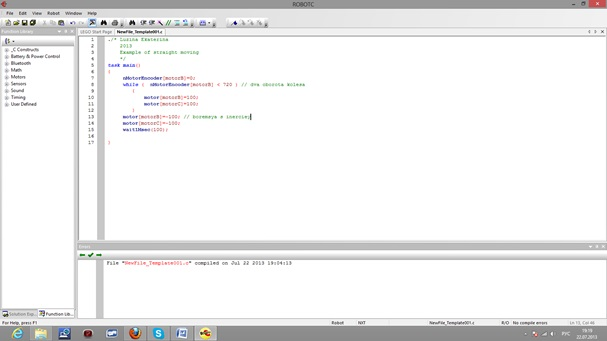
\includegraphics[width=1\linewidth]{chapters/chapter10/images/1}
		\caption{}
		\label{ris:image10x1}
	\end{center}
\end{figure}

Можно заметить, что для удобства пользователя, разные по смыслу блоки автоматически пишутся разны цветом: комментарии зеленым, синим функции и процедуры, бордовым~--- переменные.